\subsection{Theoretical graph of the molar mass versus conversion}

    \begin{figure}[H]
        \centering
        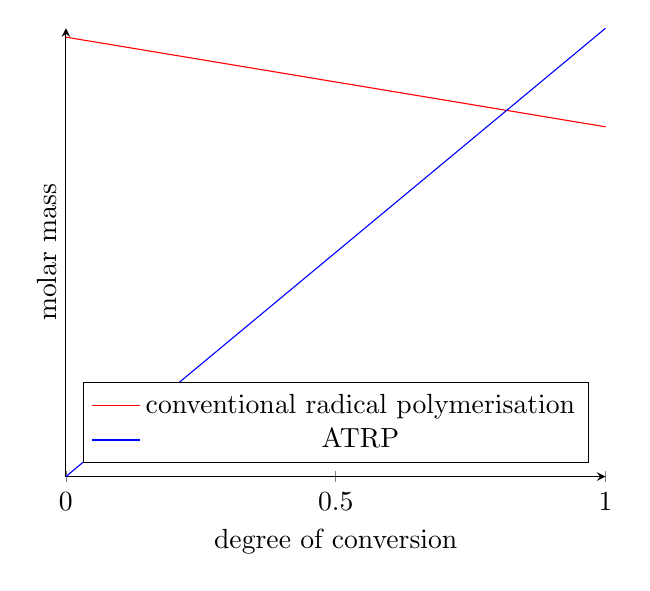
\begin{tikzpicture}
            \begin{axis}[
                ymajorticks=false,
                xtick={0,0.5,1},
                axis lines = left,
                xlabel = degree of conversion,
                ylabel = molar mass,
                legend pos=south east,
            ]
            %Below the red parabola is defined
            \addplot [
                domain=-0:1, 
                samples=10, 
                color=red,
            ]
            {0.98-0.2*x};
            \addlegendentry{conventional radical polymerisation}
            %Here the blue parabola is defined
            \addplot [
                domain=-0:1, 
                samples=10, 
                color=blue,
                ]
                {x};
            \addlegendentry{ATRP}
            
            \end{axis}
            \end{tikzpicture}
            \caption{Theoretical graph}  
    \end{figure}



    